% !TeX root = ../main.tex
\chapter{Pregled korištenog skupa podataka}
U ovom poglavlju opisan je skup podataka korišten u radu, s naglaskom na njegovu strukturu, anotacije i scenarije vožnje koje sadrži. Posebna pozornost posvećena je DADA-2000\supercite{dada2000github} skupu, jer upravo taj set omogućuje obradu stvarnih prometnih situacija i procjenu ponašanja sustava u različitim uvjetima. Također je prikazano kako su podaci lokalno organizirani, kako se gradi indeks te prema kojim kriterijima su odabrani uzorci za daljnju obradu i evaluaciju. Iako se termin \textit{dataset} češće koristi kada se govori o treniranju modela dubokog učenja, u ovom radu koristimo ovaj \textit{dataset} radi bogate biblioteke koja pokriva velik broj slučajeva sudara ili bliskih sudara na kojima je moguće testirati model.

\section{DADA-2000 skup podataka}
DADA-2000 je skup podataka usmjeren na prometne scenarije nesreća i bliskih nesreća, razvijen za istraživanje ponašanja sustava u kritičnim situacijama vožnje. Posebna vrijednost skupa je u tome što obuhvaća dinamične i neravnomjerno zastupljene kategorije događaja, zbog čega je prikladan za testiranje robusnosti ADAS pipelinea u realnim uvjetima. Iako je izvorno predstavljen u kontekstu predviđanja vozačeve pažnje, u ovom radu koristi se kao praktična osnova za evaluaciju detekcije traka, prepreka i procjene rizika sudara u različitim scenama. Takav izbor omogućuje provjeru sustava na zahtjevnim primjerima koji su relevantni za stvarnu cestovnu primjenu.

\subsection{Struktura podataka}
DADA-2000 dataset organiziran je u numerirane kategorije od kojih svaka ili više njih predstavlja vrstu incidenta. Pa tako razlikujemo kategorije:
\begin{itemize}
    \item 1, 3, 5, 7, 10 -- prelaženje ceste
    \item 2, 4, 6, 8, 11, 13--18 -- sudar
    \item 9, 12 -- pretjecanje
    \item 19--36 -- gubitak kontrole ili sudar
    \item 37, 58, 59 -- pad
    \item 47, 49, 51 -- grebanje
    \item 38, 40, 43, 45, 48, 50, 52--57, 60 -- udarac
    \item 39, 42, 61 -- gubitak kontrole
    \item 41, 44, 62 -- kvar komponenata
\end{itemize}
\begin{figure}[H]
    \centering
    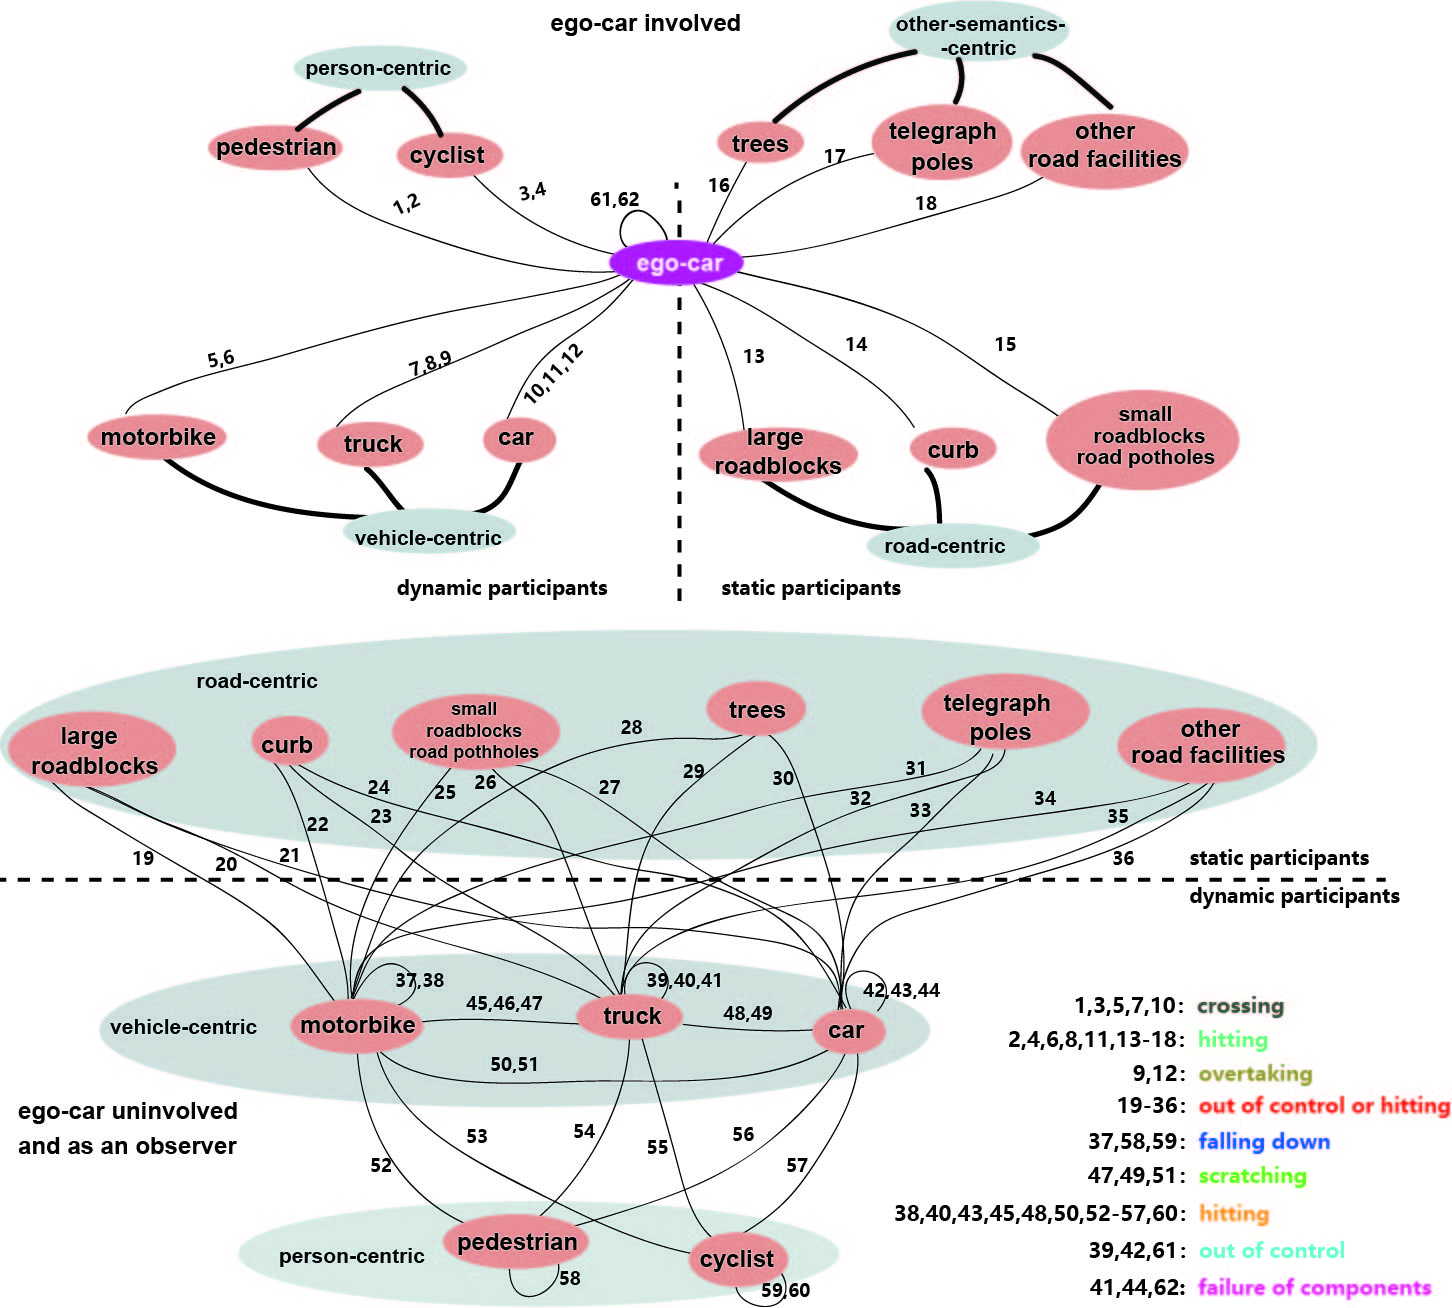
\includegraphics[width=0.85\linewidth]{figures/accident_classification.jpg}
    \caption{Kategorije incidenata u skupu DADA-2000.\supercite{dada2000github}}
    \label{fig:dada_categories}
\end{figure}

\subsection{Anotacije i oznake}
Anotacije u DADA-2000 zapisu nalaze se u CSV tablici gdje svaki red predstavlja jedan video-zapis i njegov opis kroz unaprijed definirane stupce. Zaglavlje eksplicitno definira kodirane kontekstne oznake: \textit{weather (sunny, rainy, snowy, foggy) 1--4}, \textit{light (day, night) 1--2}, \textit{scenes (highway, tunnel, mountain, urban, rural) 1--5} i \textit{linear (arterials, curve, intersection, T-junction, ramp) 1--5}. Uz to su navedeni \textit{type}, binarna oznaka \textit{whether an accident occurred (1/0)}, okvirni markeri \textit{abnormal start frame}, \textit{accident frame}, \textit{abnormal end frame}, \textit{total frames} te intervalni stupci \textit{[0,tai]}, \textit{[tai,tco]}, \textit{[tai,tae]}, \textit{[tco,tae]} i \textit{[tae,end]}. Na kraju svaki zapis sadrži i tekstualna polja \textit{texts}, \textit{causes} i \textit{measures}, koja opisuju događaj, uzrok i preporučenu mjeru.

\subsection{Uvjeti snimanja i scenariji}
Uvjeti snimanja u DADA-2000 označeni su atributima \textit{weather} (sunčano, kiša, snijeg, magla) i \textit{light} (dan/noć). Kontekst vožnje opisan je stupcima \textit{scenes} (autocesta, tunel, planinsko, urbano i ruralno okruženje) te \textit{linear} (arterija, zavoj, raskrižje, T-raskrižje, rampa). Svaki zapis dodatno sadrži tip incidenta (\textit{type}) i oznaku je li nesreća nastupila (\textit{1/0}), pa je moguće analizirati scenarije kroz različite kombinacije uvjeta.

\section{Organizacija lokalnih podataka}
Podtci DADA-2000 skupa organizirani su unutar lokalnog projekta radi jednostavnijeg učitavanja, pretraživanja i obrade. Naglasak je na praktičnom tijeku rada: od izgradnje lokalnog indeksa, preko učitavanja i pregleda videozapisa, do odabira podskupova za buduće testove.

\subsection{Izgradnja lokalnog indeksa}
Lokalni indekser uveden je kako bi se rad sa skupom DADA-2000 ubrzao i standardizirao prije same obrade videa. Umjesto da sustav pri svakom pokretanju ponovno prolazi kroz cijelu strukturu direktorija i ručno usklađuje zapise iz CSV anotacija, indekser jednom prolazi kroz dataset, prikuplja metapodatke o zapisima i sprema ih u SQLite\supercite{sqlite} bazu s dvije povezane tablice (zapisi i anotacije). Ključ povezivanja je kombinacija kategorije i video ID-a, pa se odmah može označiti je li zapis ispravno uparen, nedostaje li anotacija ili je ključ dvosmislen. Takav pristup omogućuje brže dohvaćanje pojedinog videa, filtriranje po kategoriji i direktni dohvat spojenih podataka bez ponovnog parsiranja izvora. Dodatno, izgradnja indeksa radi atomski (privremena baza pa zamjena), što smanjuje rizik od djelomično zapisanih ili nekonzistentnih podataka. Bez ovog koraka pipeline bi bio sporiji, osjetljiviji na greške u mapiranju i teže ponovljiv između različitih pokretanja.

\subsection{Učitavanje i pregled videa}
Učitavanje videa u projektu kreće od lokalnog indeksa: za zadani \textit{category\_id} i \textit{video\_id} dohvaća se točan zapis i putanja do podataka, a zatim se po potrebi preusmjeri na mapu \textit{images} ako je zapis inicijalno vezan uz pomoćne mape poput \textit{fixation} ili \textit{maps}. Okviri se zatim iteriraju preko parsera koji podržava i sekvence slika i video datoteke, pri čemu se svaki okvir referencira kroz \textit{frame\_ref} i učitava tek kada je potreban. U scenarijskom pokretanju odabrani video se unaprijed predmemorira u RAM, što omogućuje stabilniji prikaz, brže pomicanje po frameovima i manje oscilacije zbog ponovljenih pristupa disku. Za pregled i provjeru zapisa koristi se poseban player koji nad okvirom prikazuje i oznaku stanja (\textit{normal}, \textit{abnormal}, \textit{accident\_frame}) na temelju anotiranih granica događaja.